% Copyright (c) 2021-2024 Michael Kuhn
%
% Permission to use, copy, modify, and/or distribute this software for any
% purpose with or without fee is hereby granted.
%
% THE SOFTWARE IS PROVIDED "AS IS" AND THE AUTHOR DISCLAIMS ALL WARRANTIES WITH
% REGARD TO THIS SOFTWARE INCLUDING ALL IMPLIED WARRANTIES OF MERCHANTABILITY
% AND FITNESS. IN NO EVENT SHALL THE AUTHOR BE LIABLE FOR ANY SPECIAL, DIRECT,
% INDIRECT, OR CONSEQUENTIAL DAMAGES OR ANY DAMAGES WHATSOEVER RESULTING FROM
% LOSS OF USE, DATA OR PROFITS, WHETHER IN AN ACTION OF CONTRACT, NEGLIGENCE OR
% OTHER TORTIOUS ACTION, ARISING OUT OF OR IN CONNECTION WITH THE USE OR
% PERFORMANCE OF THIS SOFTWARE.

\documentclass[
	aspectratio=169,
	compress,
]{beamer}

\usetheme{Magdeburg}

\usepackage[T1]{fontenc}
\usepackage[utf8]{inputenc}

\usepackage{libertinus}
\usepackage[varqu,scaled=0.95]{inconsolata}
\usepackage{newtxmath}

\usepackage[english]{babel}

\usepackage{appendixnumberbeamer}
\usepackage{graphicx}
\usepackage[htt]{hyphenat}
\usepackage{listings}
\usepackage{microtype}
\usepackage{subcaption}
% Required for listings's upquote
\usepackage{textcomp}
\usepackage{upquote}
\usepackage{xcolor}

\usepackage[capitalise,noabbrev]{cleveref}

\usepackage[color=ovgu-orange]{todonotes}

\usepackage{lipsum}

\newenvironment{graytext}{\color{ovgu-lightgray}}{\ignorespacesafterend}

\graphicspath{{./figures/}}

% \lstset{
% 	basicstyle=\ttfamily\small,
% 	commentstyle=\color{ovgu-darkgray},
% 	keywordstyle=\color{ovgu-blue},
% 	numberstyle=\ttfamily\small\color{ovgu-darkgray},
% 	stringstyle=\color{ovgu-purple},
% 	rulecolor=\color{ovgu-lightgray},
% 	frame=single,
% 	numbers=left,
% 	language=C,
% 	breaklines=true,
% 	breakatwhitespace=true,
% 	postbreak=\hbox{$\hookrightarrow$ },
% 	showlines=true,
% 	showstringspaces=false,
% 	upquote=true,
% 	tabsize=4,
% 	gobble=4,
% 	captionpos=b,
% 	abovecaptionskip=\medskipamount,
% }

\newcommand{\navframetitle}[1]{\frametitle{#1\hfill{\footnotesize\lastsection{}}}}

% \title{Graph Traversal Languages for \\Large-Scale Graph Processing on\\ Modern Hardware}
% \subtitle{Kickoff Presentation}
\title{Graph Traversal Languages}
\subtitle{for Large-Scale Graph Processing\\on Modern Hardware}

\author[Pascal Zittlau]{
Pascal Zittlau\\
{\footnotesize\href{mailto:pascal.zittlau@ovgu.de}{\nolinkurl{pascal.zittlau@ovgu.de}}}
}

\date{\today}

\institute{
Faculty of Computer Science\\
Otto von Guericke University Magdeburg \\\\ 
{16th Student Conference on Software Engineering and Database Systems}\\
{Supervisor: Paul Blockhaus}
}

\titlegraphic{\vspace{0.5cm}\hfill
\includegraphics[width=0.375\textwidth]{OVGU-INF}}

% \AtBeginSection[]{
% 	\begin{frame}[plain,noframenumbering]
% 		\frametitle{Outline}
%
% 		\tableofcontents[currentsection]
% 	\end{frame}
% }

% \AtBeginSubsection[]{}

\begin{document}

\maketitle

\section{Introduction}
\label{sec:introduction}

\begin{frame}
	\navframetitle{Relevance}

	\begin{columns}[T]
		\begin{column}{0.6\textwidth}
	\textbf{Why is it relevant?}
	\begin{itemize}
		\item Ubiquity of Graphs
		\item Massive datasets
		\item Hardware Evolution
	\end{itemize}
	\bigskip
    \textbf{Key Problem:}\\\hspace{1.6em} How effectively do high-level graph\\\hspace{1.6em} languages map to optimized execution\\\hspace{1.6em} on diverse, modern hardware?
        \end{column}
		\begin{column}{0.4\textwidth}
            \begin{figure}
                \centering
                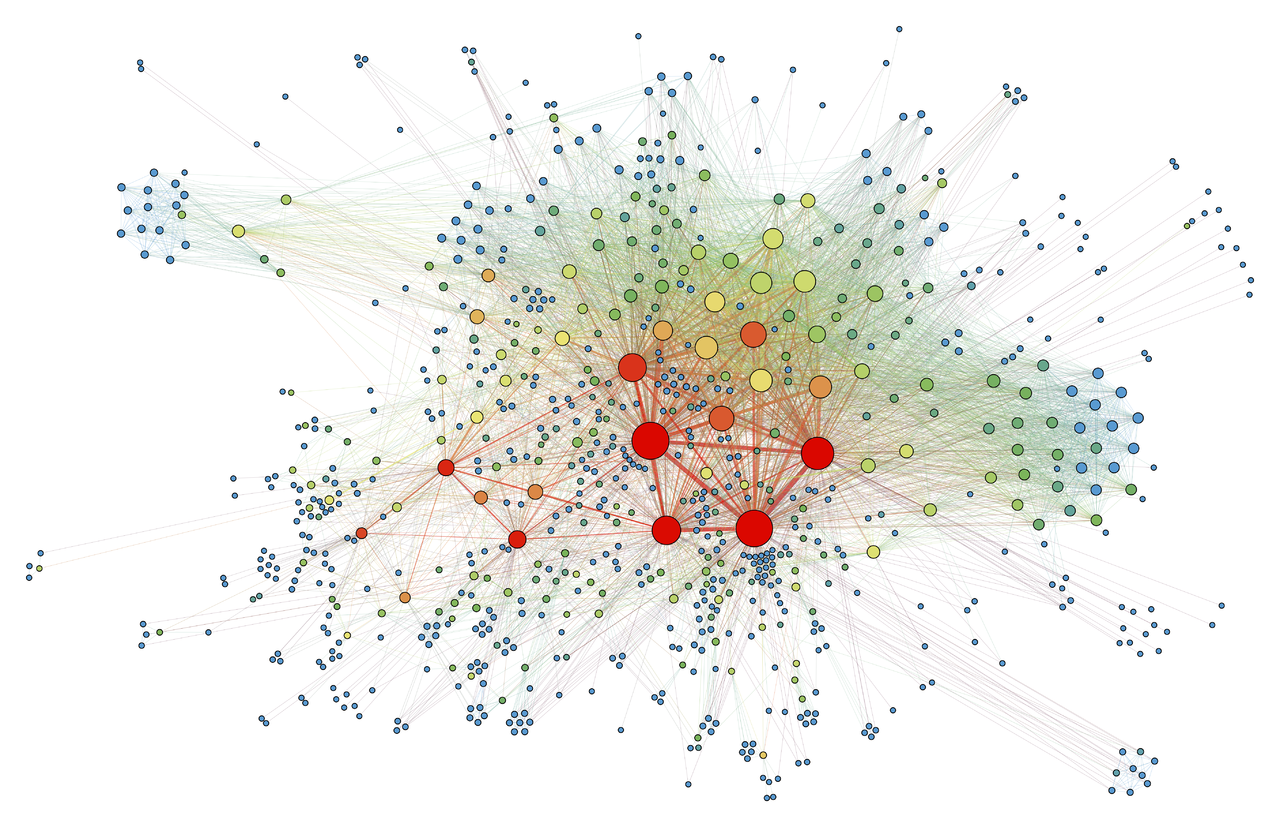
\includegraphics[width=0.95\textwidth]{./figures/SocialNetworkAnalysis.png}
                \captionsetup{justification=centering}
                \caption{A sample Social Graph \cite{WikimediaSocialGraph}}
                \label{fig:socialGraph}
            \end{figure}
        \end{column}
	\end{columns}
\end{frame}

\begin{frame}
	\navframetitle{Topic}

	\begin{columns}[T]
		\begin{column}{0.5\textwidth}
	\textbf{What is the survey about?}
	\begin{itemize}
		\item Querying \textbf{large-scale graphs} 
        \begin{itemize}
            \item RDF and Property Graphs
        \end{itemize}
		\item Surveying \textbf{graph query languages}
        \begin{itemize}
            \item SPARQL, Cypher, Gremlin, GQL
        \end{itemize}
		\item Performance on \textbf{modern hardware}
            \begin{itemize}
                \item Multi-core CPUs, GPUs, FPGAs, \dots
            \end{itemize}
	\end{itemize}
        \end{column}
		\begin{column}{0.5\textwidth}
            \begin{figure}
                \centering
                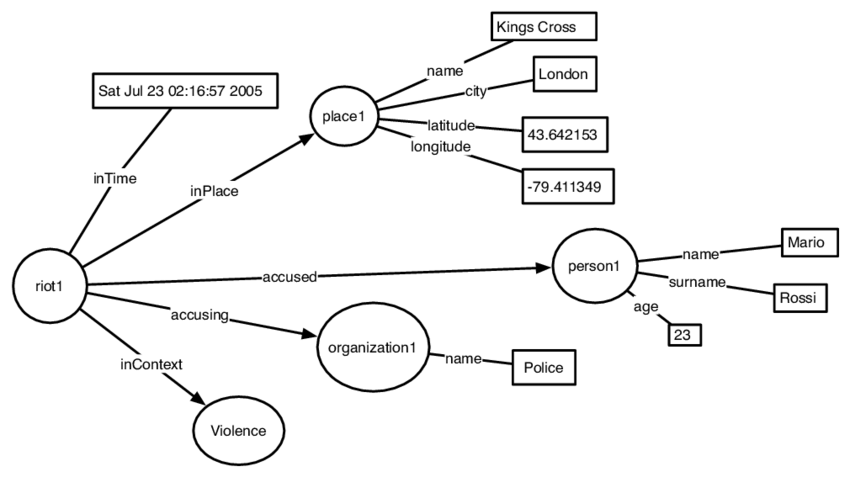
\includegraphics[width=0.95\textwidth]{./figures/rdf_graph.png}
                \captionsetup{justification=centering}
                \caption{Example of a RDF Graph \cite{VincenzoSemanticReasoner}}
                \label{fig:rdfGraph}
            \end{figure}
        \end{column}
	\end{columns}

\end{frame}


\section{Scope and Literature}
\label{sec:background}

\begin{frame}[fragile]
	\navframetitle{Scope}

	\begin{columns}[T]
		\begin{column}{0.4\textwidth}
\vspace{2em}
			\textbf{Key Areas of Investigation:}
			\begin{itemize}
				\item Traversal \& Pattern Matching
				\item Parallel Execution % (CPU/GPU)
				\item Hardware Acceleration % (SIMD, FPGA, CSD)
				\item Algorithm Integration % (Shortest Path, PageRank)
                \begin{graytext}
				\item Backend Abstractions % (GraphBLAS)
				\item Query Optimization
                \end{graytext}
			\end{itemize}
		\end{column}
		\begin{column}{0.6\textwidth}
                \centering
            \begin{figure}
                \centering
                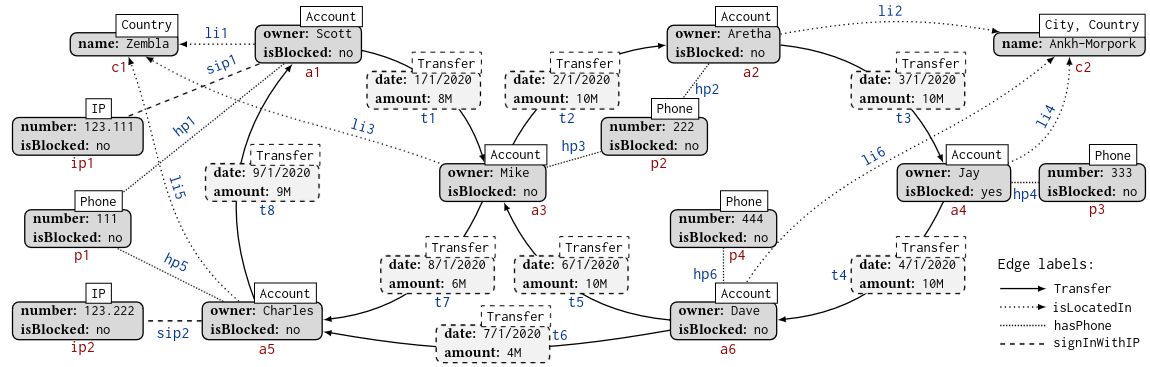
\includegraphics[width=0.95\textwidth]{./figures/propertyGraph.png}
                \captionsetup{justification=centering}
                \caption{Example of a labelled Property Graph \cite{DBLP:GraphPatternMatchinginGQL}}
                \label{fig:propertyGraph}
            \end{figure}
            \vspace{-1em}
                \begin{lstlisting}[language=,basicstyle=\tiny,caption={Cypher Query on graph in \cref{fig:propertyGraph}},captionpos=b,backgroundcolor=\color{white}]
MATCH (a:Account {isBlocked:'no'})-[:isLocatedIn]->
      (g: City {name:'Ankh-Morpork'})<-[:isLocatedIn]-
      (b:Account {isBlocked:'yes'}),
      p = (a)-[:Transfer*1..]->(b)
RETURN a.owner
                \end{lstlisting}
		\end{column}
	\end{columns}
\end{frame}

\begin{frame}
	\navframetitle{Academic Sources and Standards}
    \vspace{-1em}
	\begin{columns}[T]
		\begin{column}{0.3\textwidth}
            \begin{figure}
                \captionsetup{font={scriptsize}}
                \caption{\cite{FoundationsOfModernQueryLanguages}}
                \begin{center}
                    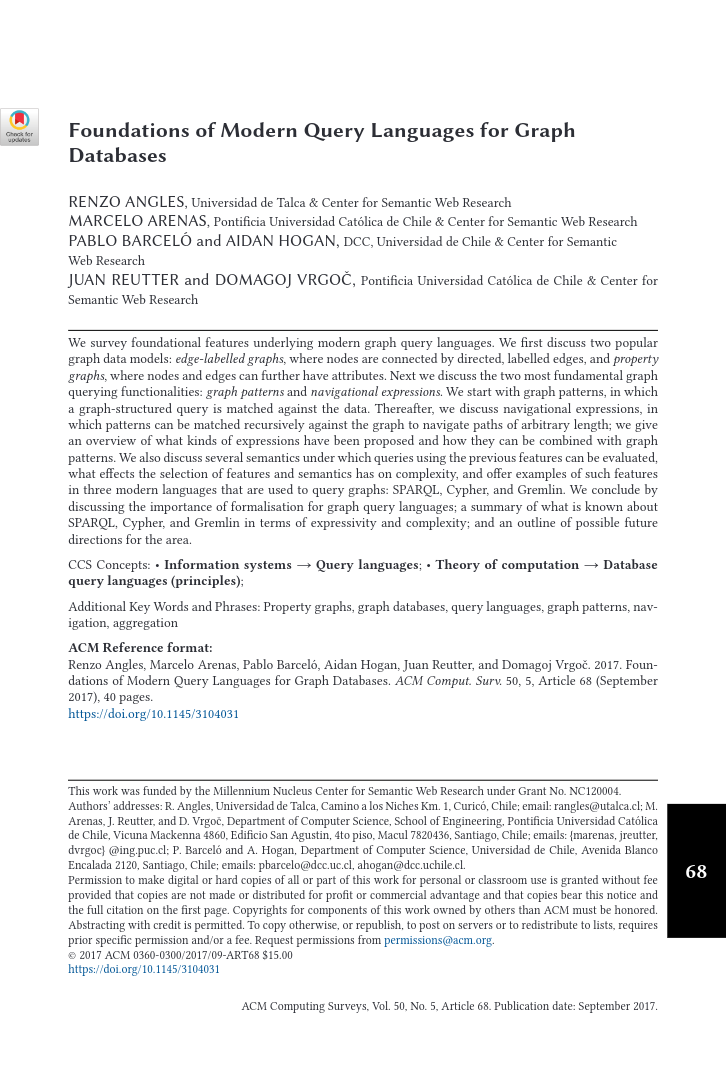
\includegraphics[width=\textwidth]{./figures/foundationOfModernQueryLanguages.png}
                \end{center}
            \end{figure}
        \end{column}
        \pause
		\begin{column}{0.3\textwidth}
            \begin{figure}
                \captionsetup{font={scriptsize}}
                \caption{\cite{DBLP:GraphPatternMatchinginGQL}}
                \begin{center}
                    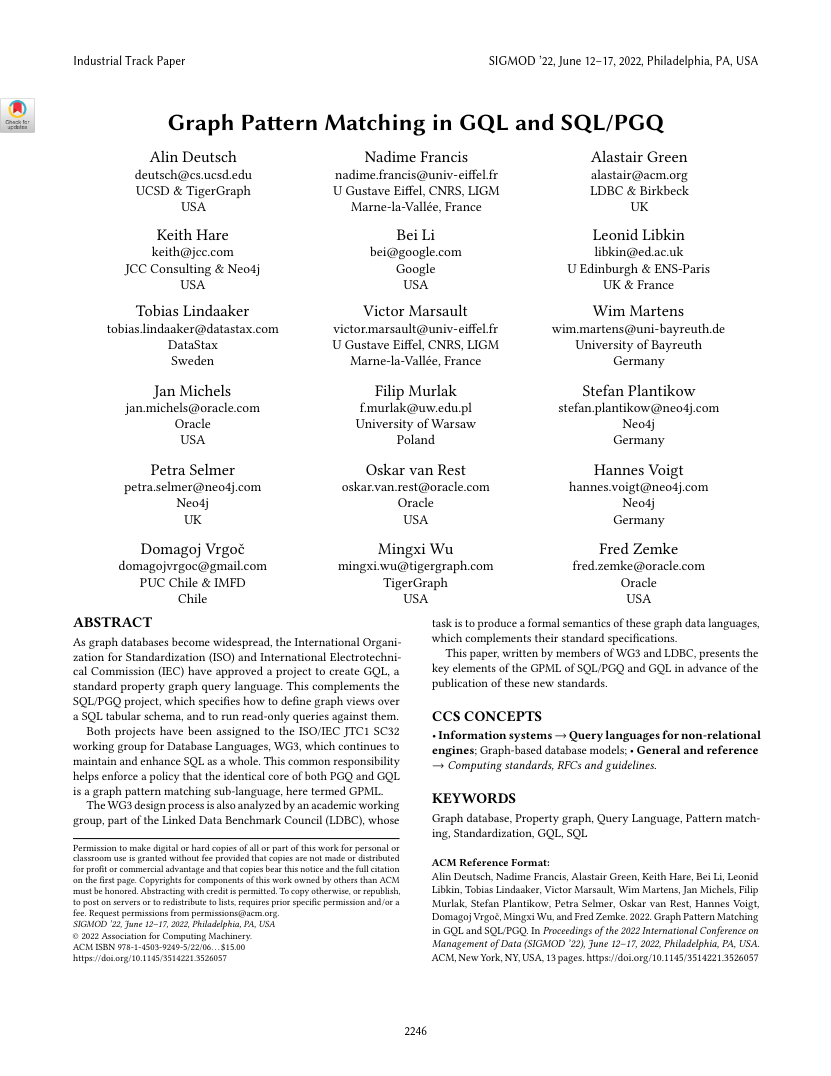
\includegraphics[width=\textwidth]{./figures/graphPatternMatchingGQL.png}
                \end{center}
            \end{figure}
        \end{column}
        \pause
		\begin{column}{0.3\textwidth}
            \begin{figure}
                \captionsetup{font={scriptsize}}
                \caption{\cite{SPARQLDocs}}
                \begin{center}
                    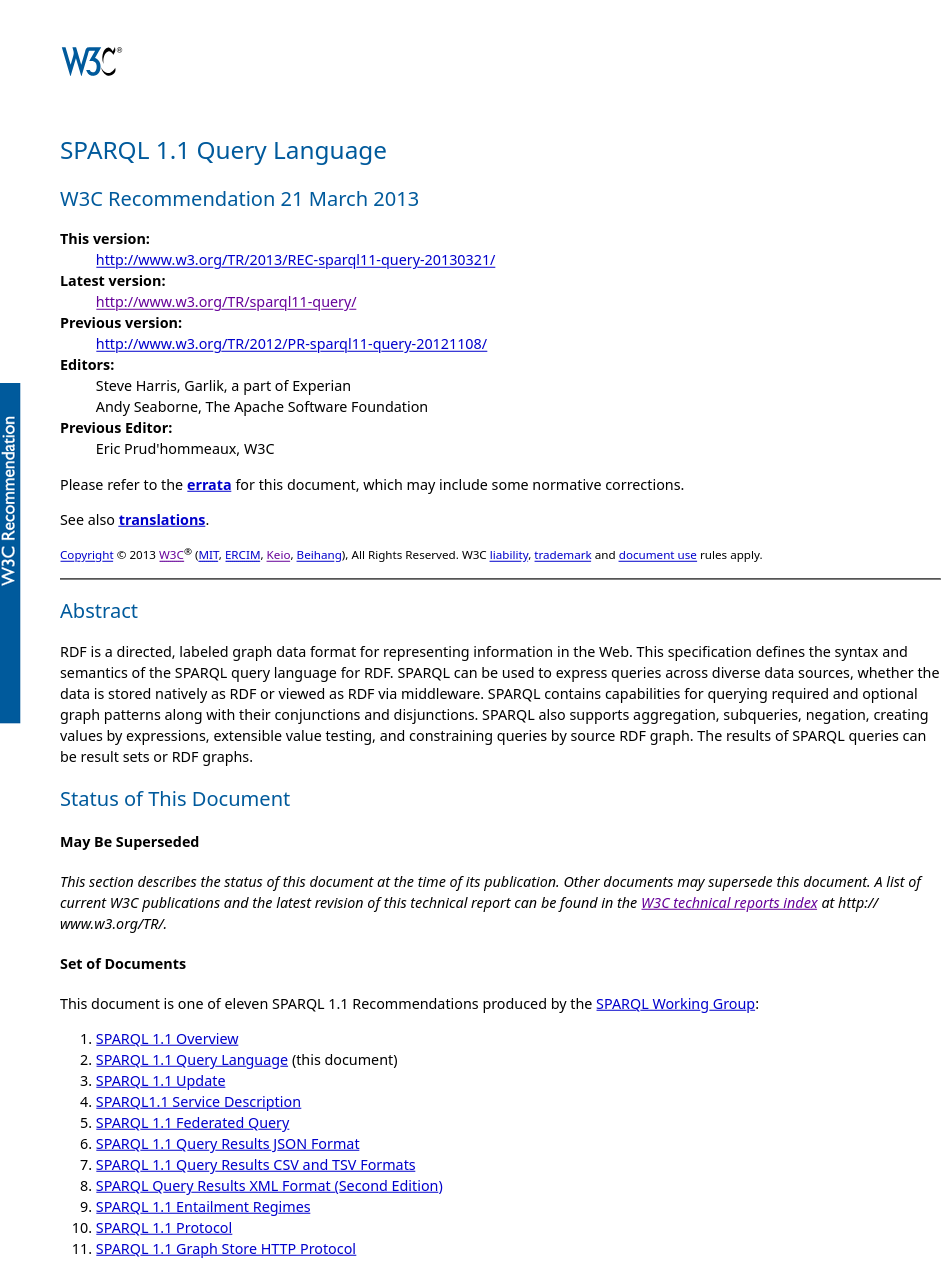
\includegraphics[width=\textwidth]{./figures/sparqlDocs.png}
                \end{center}
            \end{figure}
        \end{column}
    \end{columns}
\end{frame}

\begin{frame}
	\navframetitle{Industry Sources}
    \vspace{-1em}
	\begin{columns}[T]
		\begin{column}{0.3\textwidth}
            \begin{figure}
                \captionsetup{font={scriptsize}}
                \caption{\cite{neo4jSparkLoader}}
                \begin{center}
                    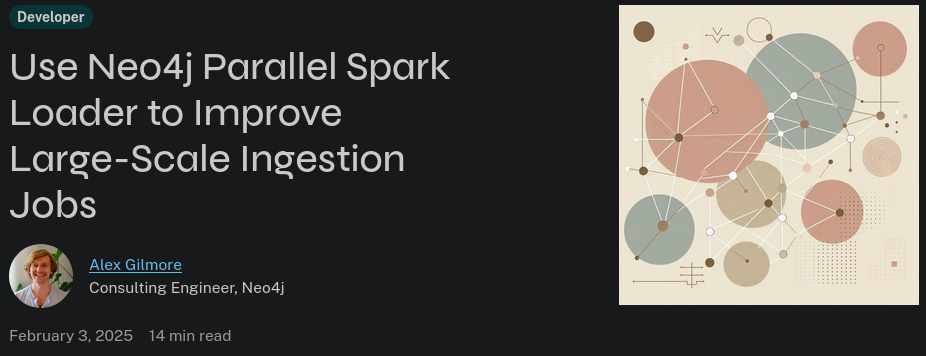
\includegraphics[height=0.2\textheight]{./figures/neo4jSpark.png}
                \end{center}
            \end{figure}
            \begin{figure}
                \captionsetup{font={scriptsize}}
                \caption{\cite{neo4jCypherGOL}}
                \begin{center}
                    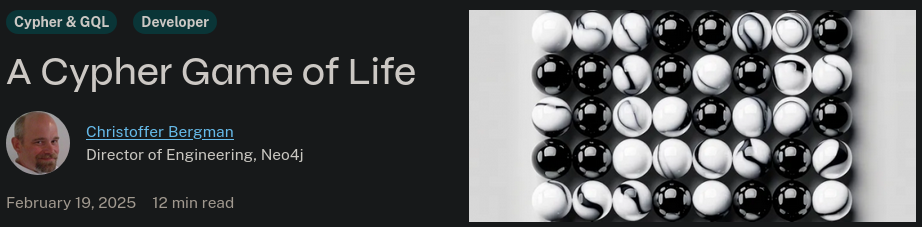
\includegraphics[width=\textwidth]{./figures/neo4jCypherGameOfLife.png}
                \end{center}
            \end{figure}
        \end{column}
        \pause
		\begin{column}{0.3\textwidth}
            \begin{figure}
                \captionsetup{font={scriptsize}}
                \caption{\cite{MemgraphDocs}}
                \begin{center}
                    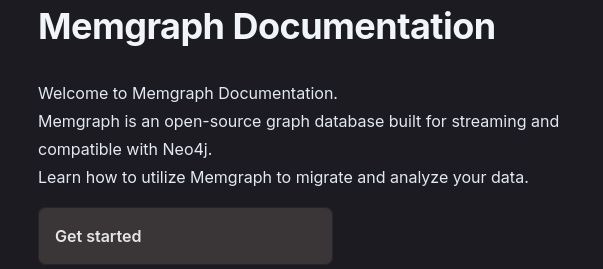
\includegraphics[height=0.2\textheight]{./figures/memgraphDocs.png}
                \end{center}
            \end{figure}
            \begin{figure}
                \captionsetup{font={scriptsize}}
                \caption{\cite{MemgraphSkipList}}
                \begin{center}
                    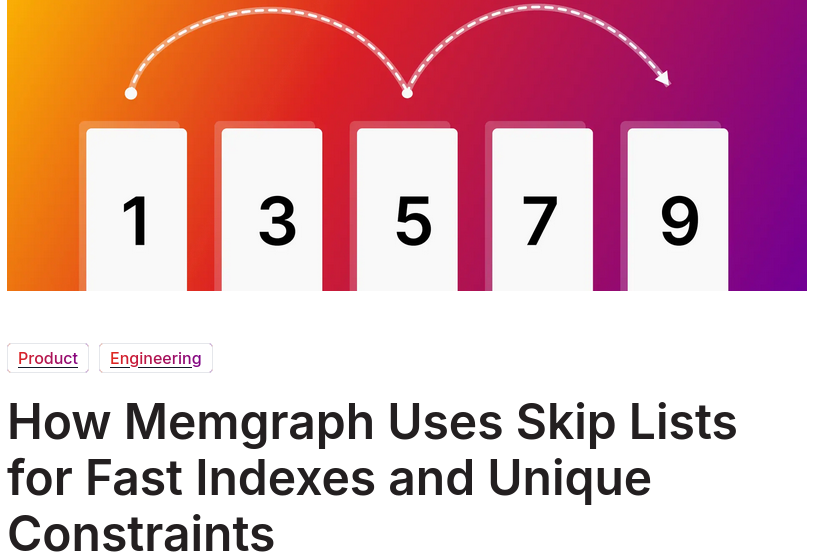
\includegraphics[width=\textwidth]{./figures/memgraphSkip.png}
                \end{center}
            \end{figure}
        \end{column}
        \pause
		\begin{column}{0.3\textwidth}
            \begin{figure}
                \captionsetup{font={scriptsize}}
                \caption{\cite{kuzudbWCOJ}}
                \begin{center}
                    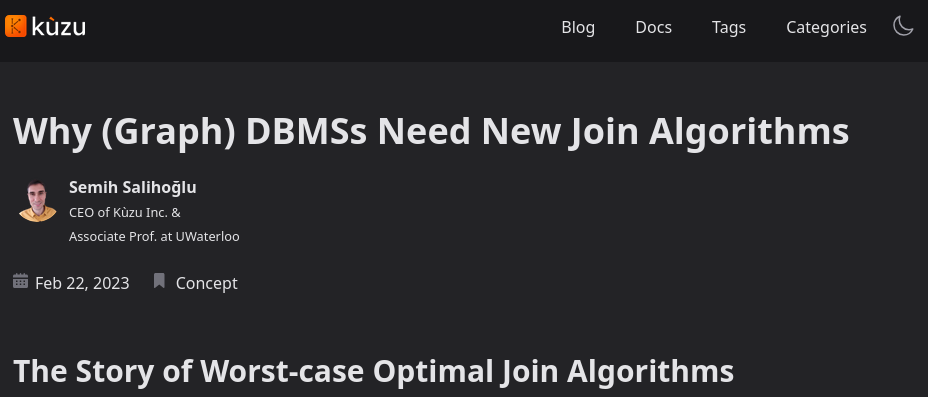
\includegraphics[height=0.2\textheight]{./figures/kuzuWCOJ.png}
                \end{center}
            \end{figure}
            \begin{figure}
                \captionsetup{font={scriptsize}}
                \caption{\cite{kuzudbFactorization}}
                \begin{center}
                    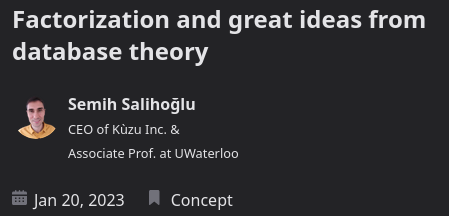
\includegraphics[width=\textwidth]{./figures/kuzuFactorization.png}
                \end{center}
            \end{figure}
        \end{column}
    \end{columns}
\end{frame}

\section{Methodology}
\label{sec:methodology}

\begin{frame}
	\navframetitle{Structure \& Discussion Approach}

	\begin{columns}[T]
		\begin{column}{0.5\textwidth}
			\textbf{Planned Paper Structure:}
			\begin{enumerate}
                \item Introduction
                \item Background on Data Models
                \item Established Languages Overview
                \item Upcoming Standards Languages
                \item Parallelization \& Hardware Acceleration
                \item \textcolor{ovgu-lightgray}{Optimization \& Backends}
                \item Algorithm Integration
                \item Synthesis: State-of-the-Art, Challenges,\\\hspace{4.3em} Future Directions
			\end{enumerate}
		\end{column}
		\begin{column}{0.5\textwidth}
        % TODO: some kind of image
		\end{column}
	\end{columns}

\end{frame}

\section{Conclusion}
\label{sec:conclusion}

\begin{frame}
	\navframetitle{Conclusion \& Questions}

    \textbf{Recap:} Surveying graph traversal languages, focusing on mappings to modern\\\hspace{3.05em} hardware for large-scale processing.

    \textbf{Goal:} Provide a structured overview of the state-of-the-art,\\\hspace{2.5em} identifying key challenges and opportunities.

	\vfill % Pushes content up and leaves space below

    \pause

	\centering
	\Large Thank you!

    \pause

	\bigskip
	\normalsize Questions?

\end{frame}

\appendix

\AtBeginSection[]{}
\AtBeginSubsection[]{}

\section{References}

\begin{frame}[allowframebreaks]
	\frametitle{References}

	\bibliographystyle{apalike}
	\bibliography{presentation}
\end{frame}

\end{document}
